\chapter{Theorie}\label{chap:background}
Im folgenden soll der theoretische Hintergrund bezüglich der 
Betrachteten Probleme sowie die theoretische Funktionsweise des 
Detektors betrachtet werden. 

\section{Routinen}\label{Chap:Back-Sec:Routine}
Bei Go-Routinen handelt es sich um leichtgewichtige Threads, welche 
nebenläufig mit anderen Routinen auf dem selben Adressraum laufen~\cite{effectiveGo}.
Anders als Threads in vielen anderen Programmiersprachen werden sie nicht 
durch den OS-Kernel, sondern durch die Go-Runtime selber gesteuert.
Diese besitzt einen eigenen Scheduler, welcher eine Technik namens $m$:$n$-Scheduling 
verwendet, um durch Multiplexing $m$ Go-Routinen auf $n$ OS-Threads auszuführen.
Diese Herangehensweise hat den Vorteil, dass dadurch eine bessere Ausführungsgeschwindigkeit 
erreicht und ein geringerer Speicher benötigt wird. Dadurch ist 
es möglich, dass tausende oder sogar hunderttausende Routinen gleichzeitig 
auf einer Routine laufen. Sie erleichtert außerdem 
die Implementierung von Synchronisations- und Kommunikationsmechanismen.

\section{Mutexe}\label{Chap:Back-Sec:Mutex}
Mutexe (auch Locks genannt) gehören zu den am weitesten verbreitenten Mechanismen 
zur Synchronisierung nebenläufiger Programme~\cite{Undead}. Sie bilden 
eine Lösung für das Problem des kritischen Abschnitts. In solch einem 
kritischen Abschnitt darf sich immer nur maximal eine Routine gleichzeitig
aufhalten. Solche Abschnitte werden nun mit einem Mutex umschlossen. 
Sie werden unter anderem verwendet um zu verhindern, dass 
mehrere Routinen gleichzeitig auf die selbe globale Datenstruktur 
zugreifen. Mutexe besitzen zwei Zustände, geöffnet und geschlossen, mit denen 
ihre Verhalten gesteuert wird.
Sie besitzen dabei die folgenden Operationen:
\begin{itemize}
  \item Lock: Die Lock-Operation wird vor dem Eintritt in einen kritischen 
    Bereich aufgerufen. Sie versucht den Mutex zu schließen. Ist es momentan 
    geöffnet, wird der Mutex geschlossen und der kritische
    Bereich ausgeführt. Ist der Mutex bereits geschlossen, dann muss 
    die Routine, in welcher die Lock-Operation ausgeführt 
    werden soll so lange warten, bis der Mutex wieder geöffnet wird und 
    geschlossen werden kann.
  \item TryLock: Eine TryLock Operation versucht, wie die Lock-Operation,
    einen Mutex zu schließen. Anders als bei Lock wird die Routine allerdings 
    nicht blockiert, wenn eine Schließung nicht direkt möglich ist. Es wird 
    lediglich zurückgegeben, ob sie erfolgreich war oder nicht. Ein Programmierer 
    kann in diesem Fall selber entscheiden, wie das Programm weiter ablaufen 
    soll, ob also z.B. der kritische Bereich übersprungen werden soll.
  \item Unlock: Diese Operation öffnet einen geschlossenen Mutex. Der Versuch ein 
    geöffnetes Mutex zu öffnen führt zu einem Laufzeitfehler. 
    Theoretisch verhalten sich Mutexe in Go wie binäre Semaphore, d.h.~es ist möglich, 
    dass eine Routine ein 
    geschlossenes Mutex freigibt, obwohl das Mutex von einer anderen Routine
    geschlossen wurde. Da dies in der Praxis sehr leicht zu einem 
    unvorhersehbaren Verhalten führen kann, ist es fast immer üblich, 
    ein Mutex immer nur von derjenigen Routine freizugeben, von der es beansprucht wurde. 
    Im weiteren wird daher angenommen, 
    dass ein Mutex immer von der Routine geöffnet wird, von welchem es 
    geschlossen wurde.
\end{itemize}
Mutexe können mit (Try)RLock Operationen zu RW-Mutex erweitert werden.
Dabei kann der selbe Mutex von mehreren 
(Try)RLock-Operationen geschlossen werden, ohne dass es zwischenzeitlich
geöffnet werden muss. Es ist allerdings 
nicht möglich, dass ein Mutex gleichzeitig über eine RLock- und eine Lock-Operation 
geschlossen wird. RW-Mutexe können z.B. verwendet werden, wenn mehrere Routinen 
gleichzeitig lesend auf eine Datenstruktur zugreifen dürfen, allerdings nur, 
wenn gerade keine Routine schreibend auf die selbe Datenstruktur zugreift.


\section{Channel}\label{Chap:Back-Sec:Chann}
Channel~\cite{effectiveGo} ermöglichen es Routinen untereinander zu 
kommunizieren.
Ein Channel \texttt{c} kann Daten \texttt{d} senden (\texttt{c} <- \texttt{d})
und empfangen (<- \texttt{c}). Das genaue Verhalten der Channel hängt dabei 
davon ab, ob es sich um einen gebufferten oder ungebufferten Channel handelt. \\
Bei einem ungebufferten Channel müssen Send- und Receive-Operation gleichzeitig 
ablaufen. Möchte eine Routine \texttt{R} Daten auf einem Channel \texttt{c} senden, 
ist aber keine Routine bereit die Daten von \texttt{c} zu empfangen, 
dann muss \texttt{R} so lange warten, bis eine andere Routine ein
Receive-Statement auf dem Channel \texttt{c} ausführt. Das selbe gilt auch, wenn 
eine Routine an ein Receive-Statement eines Channels kommt auf welchem 
momentan nicht gesendet wird.\\
Bei einem gebufferten Channel der Größe $n$ können bis zu $n$ Nachrichten
zwischengespeichert werden. Dies bedeutet, dass Send und Receive nicht mehr 
gleichzeitig ablaufen müssen. Eine Routine muss hierbei nur dann 
vor einer Operation warten, wenn eine Send-Operation auf einem vollen 
Channel, oder eine Receive-Operation auf einem leeren Channel ausgeführt 
wird. In allen anderen Fällen kann die Operation die Nachricht in den Buffer 
schreiben, bzw.~eine Nachricht aus dem Buffer lesen.\\
Basierend auf dem 
Go-Memory-Model gilt, dass zum einen das Senden auf einem Channel vor dem 
dazugehörigen Receive auf dem Channel synchronisiert wird und dass 
das $k$-te Receive auf einem Channel mit Kapazität $C$ vor der Beendigung
des $k+C$-ten Send auf dem Channel synchronisiert wird~\cite{memModel}.   
In der Praxis verhält sich der Buffer eines Channels allerdings wie eine FIFO-Queue,
das heißt, es wird bei einem Receive immer die ältest in dem
Buffer vorhandene Nachricht ausgegeben. Im Folgenden wird daher immer von diesem 
Verhalten ausgegangen.\\\\
Sowohl bei gebufferten als auch bei ungebufferten Channels kann es zu 
Situationen kommen, in denen mehrere Routinen gleichzeitig auf dem selben 
Channel auf eine Nachricht warten. Wird nun auf diesem Channel gesendet 
wird eine der Routinen pseudo-zufällig ausgewählt, um die Nachricht zu empfangen.\\\\
Go macht es mit der Select-Operation möglich, auf die erste von mehreren 
erfolgreichen Channel-Operationen gleichzeitig zu warten. Ein Beispiel für solch 
ein Select befindet sich in Abb.~\ref{Chan:Analyze-Sec:Channel-Fig:SelectEx}.
\begin{figure}[h!]
  \lstinputlisting{code/example_select.txt}
  \caption{Beispielprogramm für Select}
  \label{Chan:Analyze-Sec:Channel-Fig:SelectEx}
\end{figure}
In diesem Beispiel besitzt die Select-Operation 3 Cases und einen Default-Case.
Die Cases bestehen aus verschiedenen Channel-Operationen (Receive auf Channel, 
Receive auf Channel mit direkter Variablendeklaration und Send auf Channel).
Das Select-Statement probiert nun die Cases in einer zufälligen Reihenfolge 
aus. Findet es einen Case, in dem die Operation ausgeführt werden kann, wird 
die Operation, sowie der darunter stehende Block (Print-Statement) ausgeführt.
Der Default-Case wird ausgeführt, wenn keiner der anderen Cases ausgeführt 
werden kann. Er ist allerdings nicht notwendig. Besitzt das Select-Statement 
keinen Default-Case, dann blockiert die Routine so lange, bis einer der Cases 
ausgeführt werden kann.\\\\
Channel können vorzeitig durch eine \texttt{close} Operation geschlossen werden.
In diesem Fall kann auf diesem Channel nicht mehr gesendet werden. Versucht 
das Program auf einem geschlossenen Channel zu senden kommt es zu einem 
Laufzeitfehler und das Programm wird abgebrochen. Versucht das Programm 
auf einem geschlossenen Channel zu lesen, wir ein Default-Wert zurückgegeben,
ohne dass die Routine blockiert.

\section{Probleme}\label{chap:background-sec:Prob}

\subsection{Mutex}\label{Chap:Back-Sec:Prob-SubSec:Mutex}
Durch die Verwendung von Mutexen in nebenläufigen Programmen kann es 
zu sogenannten Deadlocks kommen. Blockieren sich dabei mehrere Routinen 
gegenseitig bezeichnen wir eine solche Situation als zyklisches Locking.
Abb.~\ref{Chap:Analyze-Sec:Mutex-Fig:Zyclic} zeigt ein Beispiel, in welchem es zu zyklischem 
Locking kommen kann.
\begin{figure}[h!]
  \lstinputlisting{code/zyclic-locking-example.txt}
  \caption{Beispielprogramm zyklisches Locking}
  \label{Chap:Analyze-Sec:Mutex-Fig:Zyclic}
\end{figure}
Routine 0 und Routine 1 können dabei gleichzeitig ausgeführt werden. Man betrachte den Fall, in dem 
Zeile 7 und 14 gleichzeitig ausgeführt werden, also Lock \texttt{y} von Routine 0 und Lock \texttt{x} 
von Routine 1 gehalten wird. In diesem Fall kann in keiner der Routinen die nächste Zeile ausgeführt werden,
da das jeweilige Locks, welches beansprucht werden soll bereits durch die andere Routine gehalten wird. 
Da sich diese Situation auch nicht von alleine auflösen kann, blockiert dass Programm, befindet sich also 
in einem zyklischen Deadlock.\\\\
Neben zyklischem Locking kann es auch durch doppeltes Locking von Mutexen 
zu Deadlocks kommen. Ein Beispiel dazu findet sich in 
Abb.~\ref{Chap:Analyze-Sec:Mutex-Fig:Double}.
\begin{figure}[h!]
  \lstinputlisting{code/double-locking-example.txt}
  \caption{Beispielprogramm doppeltes Locking}
  \label{Chap:Analyze-Sec:Mutex-Fig:Double}
\end{figure}
Der Mutex \texttt{x} soll hierbei mehrfach geschlossen werden, ohne dass 
es zwischenzeitlich geöffnet wird. In diesem Fall blockiert die Routine
endlos.\\\\
In Go terminiert ein Programm, wenn dessen Main-Routine terminiert, unabhängig
davon, ob andere Routinen noch laufen. Dies bedeutet, dass es nur zu einem 
``echten'' Deadlock, bei welchem das gesamte Programm blockiert, kommen kann,
wenn die Main-Routine in der Deadlock-Situation involviert ist. Sind nur 
Nicht-Main-Routinen an dem Deadlock beteiligt, kann dass Programm dennoch
terminieren. Man bezeichne Nicht-Main-Routinen, welche sich in einer blockenden 
Deadlock Situation befinden, als hängende Routinen. Auch wenn diese nicht zu einer 
nicht-terminierung des Programms führen können, handelt es sich bei ihnen dennoch 
um ungewolltes Verhalten.

\subsection{Channel}
Wie Mutexe können auch Channels zu Deadlocks führen. Diese treten auf,
wenn ein Channel auf eine Send- oder Receive-Operation wartet, ohne dass
während der Laufzeit des Programms ein Kommunikationspartner für die 
Operation gefunden wird.
Man betrachte das Programm in Abb.~\ref{Chap:Analyze-Sec:Channel-SubSec:Dangling-Fig:ExDangling}.
\begin{figure}[h!]
  \lstinputlisting{code/example-dangling-channel.txt}
  \caption{Beispielprogramm mit hängendem Channel}
  \label{Chap:Analyze-Sec:Channel-SubSec:Dangling-Fig:ExDangling}
\end{figure}
Es gibt in diesem zwei mögliche Ausführungspfade. Man betrachtet zuerst den Fall, in dem 1 mit 3 synchronisiert. 
Da eine go-Routine automatisch abgebrochen wird,  
wenn die Main-Routine terminiert, entsteht hierbei kein ``echter" Deadlock. Anders ist es, wenn 1 mit 2 synchronisiert. 
In diesem Fall wird die Main-Routine blockiert, ohne dass es eine Möglichkeit gibt, dass sie sich wieder 
befreit. Es kann also, abhängig davon, ob 1 oder 2 die Nachricht erhält zu einem Deadlock kommen. Was 
allerdings beide Fälle gemeinsam haben ist, dass sie eine Channel-Operation besitzen, welche zwar 
gestartet, allerdings nie ausgeführt wird.\\
Anders als in ungebufferten Kanälen müssen in gepufferten Kanälen Send und 
Receive einer Nachricht nicht gleichzeitig ablaufen. Hierbei kann es 
zu Situationen kommen, in dem eine Nachricht zwar erfolgreich gesendet, aber
nie ausgelesen wird. Man betrachte dazu das Beispiel in 
Abb.~\ref{Chap:Analyze-Sec:Channel-SubSec:Buffered-Fig:Ex1}.
\begin{figure}[h!]
  \lstinputlisting{code/non-read-message.txt}
  \caption{Beispielprogramm für nicht gelesenen Nachricht in gepuffertem Channel} 
  \label{Chap:Analyze-Sec:Channel-SubSec:Buffered-Fig:Ex1}
\end{figure}
Es besitzt 2 Send- aber nur eine Receive-Operation. Wäre der Channel nicht 
gepuffert, und hätte 1 mit 3 synchronisiert, würde 2 blockieren und es 
würde zu einem Deadlock, bzw. dadurch dass 2 nicht in der Main-Routine liegt
zu einer hängenden Operation kommen. Dadurch das der Channel allerdings gepuffert ist
können sowohl 1 als auch 2 senden ohne zu blockieren. Hierbei kann es nur 
zu einem blockierenden Deadlock kommen, wenn aus einem leeren Channel empfangen wird, 
ohne dass es irgendwann zu einer sendenden Operation kommt, oder wenn auf 
einem vollen Channel gesendet werden soll, ohne dass es zu einer Empfangenden
Operation kommt.\\
Anders als bei Mutexen, bei denen immer eine Lock-
und eine Unlock-Operation fest zusammen gehören können Channel-Operationen
je nach dem wie dass Programm genau anläuft verschieden Kommunikationspartner 
haben. Die Wahl der Kommunikationspaar kann außerdem, vor allem in Select-Statements
quasi non-deterministisch ablaufen, was eine Voraussage von Potenziellen 
Deadlocks deutlich verkompliziert. Aus diesem Grund beschränken wir uns 
hierbei darauf tatsächlich auftretende Probleme zu erkennen, sie zu analysieren 
und dann, soweit möglich Hinweise über die Probleme zu liefern, welche die 
Erkennung und manuelle Beseitigung der Probleme erleichtern.\\\\
Ein weiterer möglicher kritischer Fehler bei Channels liegt in dem 
Senden auf einem geschlossenen Channel. Da dies zu einem Abbruch des 
Programms führen kann. Dies sollte also unter allen Umständen vermieden werden.
Das Empfangen auf einem geschlossen Channel ist hingegeben kein Problem. 

\section{Detektor}
Der Detektor basiert auf zwei Schritten. Zuerst wird das Programm 
durchlaufen. Dabei wird ein Trace aufgezeichnet, welche die relevanten 
Informationen über den Programmablauf aufzeichnet. Dieser 
Trace wird im Anschluss analysiert, um Informationen über Probleme 
in dem Programm zu erhalten. Das ganze wird gegebenenfalls mehrfach wiederholt,
um eine breitere Abdeckung des Programmcodes zu erreichen.


\subsection{Trace}\label{chap:background-sec:trace}
Um ein Program analysieren zu können, soll der Ablauf eines Programmdurchlaufs
(Trace) aufgezeichnet werden. Der grundlegende Aufbau des Trace basiert auf~\cite{PPDP18}. 
Er wird aber um Informationen 
über Locks erweitert. Der Trace wird für jede Routine
separat aufgezeichnet. Außerdem wird, anders als in~\cite{PPDP18} ein globaler
Program-Counter für alle Routinen und nicht ein separater Counter für jede 
Routine verwendet. Dies ermöglicht es, bessere Rückschlüsse über den genauen 
Ablauf des Programms zu erziehen. Zusätzlich speichert der Trace die Anzahl 
der schon ausgeführten Send- oder Receive-Operationen für gebufferte Channel.
Die Syntax des Traces in EBNF gibt sich 
folgendermaßen:
\begin{align*}
  \begin{matrix*}[l]
    T & = & ''\ [\ '',\ \{\ U\ \},\ ''\ ]\ ''; & \text{Trace}\\
    U & = & ''\ [\ '',\ \{\ t\ \},\ ''\ ]\ ''; & \text{lokaler Trace} \\
    t & = & signal(t, i)\ |\ wait(t, i)\ |\ pre(t, as)\ |\ post(t, i, x!) & \text{Event}\\
      &   & |\ post(t, i, x?, t') |\ post(t, default)\ 
      |\ close(t, x)\  
      & \\
      &   & |\ lock(t, y, b, c) |\ unlock(t, y); & \\
    a & = & x,\ (''\ !\ ''\ |\ ''\ ?\ ''); & \\
    as & = & a\ |\ (\{\ a\ \}, [\ ''\ default\ ''\ ]); & \\
    b & = & ''-''\ |\ ''t''\ |\ ''r''\ |\ ''tr'' & \\
    c & = & ''0''\ |\ ''1''
  \end{matrix*}
\end{align*}
wobei $i$ die Id einer Routine, $t$ einen globalen Zeitstempel, $x$ die Id eines 
Channels und $y$ die Id eines Locks darstellt. Die Events haben dabei folgende Bedeutung:
\begin{itemize}
  \item \texttt{signal(t, i)}: In der momentanen Routine wurde
    eine Fork-Operation ausgeführt,
    d.h. eine neue Routine mit Id $i$ wurde erzeugt.
  \item \texttt{wait(t, i)}: Die momentane Routine mit Id $i$ wurde soeben erzeugt. Dies ist 
    in allen Routinen außer der Main-Routine das erste Event in ihrem lokalen Trace.
  \item \texttt{pre(t, as)}: Die Routine ist an einer Send- oder Receive-Operation eines 
    Channels oder an einem Select-Statement angekommen, dieses wurde aber noch nicht 
    ausgeführt. Das Argument $as$ gibt dabei die Richtung und den Channel an. 
    Ist $as = x!$, dann befindet sich der Trace vor einer Send-Operation, bei 
    $as = x?$ vor einer Receive-Operation. Bei einem Select-Statement ist 
    $as$ eine Liste aller Channels für die es einen 
    Case in dem Statement gibt. Besitzt das Statement einen Default-Case, wird
    dieser ebenfalls in diese List aufgenommen.
  \item \texttt{post(t, i, x!)}: Dieses Event wird in dem Trace gespeichert, nachdem 
    eine Send-Operation auf $x$ erfolgreich abgeschlossen wurde. 
    $i$ gibt dabei die Id der sendenden Routine an.
  \item \texttt{post(t, i, x?, t')}: Dieses Event wird in dem Trace gespeichert, nachdem 
    eine Receive-Operation des Channels $x$ erfolgreich abgeschlossen wurde. 
    $i$ gibt dabei die Id der sendenden Routine an. $t'$ gibt den Zeitstempel an,
    welcher bei dem Pre-Event der sendenden Routine galt. Durch die Speicherung der Id und des 
    Zeitstempels der sendenden Routine bei einer Receive-Operation lassen sich 
    die Send- und Receive-Operationen eindeutig zueinander zuordnen.
  \item \texttt{post(t, default)}: Wird in einem Select-Statement der Default-Case ausgeführt,
    wird dies in dem Trace der entsprechenden Routine durch $post(t, default)$ 
    gespeichert.
  \item \texttt{close(t, x)}: Mit diesem Eintrag wird das schließen eines Channels $x$ 
    in dem Trace aufgezeichnet.
  \item \texttt{lock(t, y, b, c)}: Der Beanspruchungsversuch eines Locks mit id $y$ wurde gestartet. 
    $b$ gibt dabei die Art der Beanspruchung an. Bei $b = r$ war es eine R-Lock
    Operation, bei $b = t$ eine Try-Lock Operation und bei $b = tr$ ein Try-R-Lock
    Operation. Bei einer normalen Lock-Operation ist $b = -$. Bei einer 
    Try-Lock Operation kann es passieren, dass die Operation beendet wird, 
    ohne das das Lock gehalten wird. In diesem Fall wird $c$ auf $0$, und 
    sonst auf $1$ gesetzt. Das Trace-Element wird vor der abgeschlossen 
    Beanspruchung in den Trace eingefügt um sicher zu stellen, dass 
    ein zyklisches Locking auch dann erkannt wird, wenn es zu einem 
    tatsächlichen Deadlock führt. 
  \item \texttt{unlock(t, y)}: Das Lock mit id $y$ wurde zum Zeitpunkt 
    $t$ wieder freigegeben. 
\end{itemize}


Man betrachte als Beispiel das Programm in Abb.~\ref{Chap:Tracer-Sec:Trace-Fig:Example}.\\
\begin{figure}[h]
  \lstinputlisting{code/example_code_pre.txt}
  \caption{Beispielprogramm für Tracer}
  \label{Chap:Tracer-Sec:Trace-Fig:Example}
\end{figure}
Dabei ergibt sich der folgende Trace:
\begin{align*}
  [&[signal(1, 2),\ signal(2, 3),\ signal(3, 4),\ pre(4, a?, default),\ post(5, default)]\\
  &[wait(8, 2),\ lock(9, 1, -, 1),\ pre(10, x!),\ post(16, 2, x!),\ unlock(17, 1)]\\
  &[wait(11, 3),\ pre(12, y!),\ post(13, 3, y!),\ pre(14, x?),\ post(15, 2, x?, 10)]\\
  &[wait(6, 4),\ pre(7, y?),\ post(18, 3, y?, 12)]]
\end{align*}
Aus diesem lässt sich der relevante Ablauf des Programms rekonstruieren.

\subsection{Analyze}
Nach dem das Programm durchlaufen und der Trace aufgezeichnet wurde, 
wird dieser anschließend analysiert. Dabei werden für die Erkennung von 
Problemen mit Mutexen und Channels zwei verschiedene Ansätze verwendet.

\subsubsection{Mutexe}
Man betrachte zuerst die Erkennung von zyklischem Locking. 
Da solche Situationen nur in ganz besonderen Situation auftreten 
(in Abb.~\ref{Chap:Analyze-Sec:Mutex-Fig:Zyclic} müssen Zeilen 
7 und 14 genau gleichzeitig ausgeführt werden, ohne dass Zeile 8 oder 15 ausgeführt werden), muss 
ein Detektor, welcher vor solchen Situationen warnen soll, nicht nur tatsächliche Deadlocks, sondern
vor allem potenzielle, also nicht tatsächlich aufgetretene Deadlocks erkennen. Die Erkennung der 
potenziellen Deadlocks basiert hierbei auf iGoodLock~\cite{iGoodLock} und UNDEAD~\cite{Undead}. 
Dabei wird für jede Routine ein Lock-Baum aufgebaut. Jeder in der Routine vorkommende 
(RW-)Mutex $m_i$ wird durch einen Knoten $k_i$ in dem Baum repräsentiert. 
In diesem Baum gibt es nun eine gerichtete Kante von $k_1$ nach $k_2$, wenn 
$m_1$ das
von der Routine momentan gehaltene Lock ist, welches zuletzt von der Routine 
geschlossen worden ist, währen das Lock $m_2$ geschlossen wird~\cite{lock-tree}.
Ist es nun möglich, Knoten aus verschiedenen Bäumen, welche den selben
Mutex repräsentieren so zu verbinden, dass der entstehende Graph einen Zyklus 
enthält, bedeutet dies, dass in dem Programm zyklisches Locking möglich ist. 
Man betrachte dazu das Programm in Abb.~\ref{Chap:Analyze-Sec:Mutex-Fig:ZyclicTreeCode}
\begin{figure}[h!]
  \lstinputlisting{code/example-lock-tree-code.txt}
  \caption{Beispielprogramm zyklisches Locking}
  \label{Chap:Analyze-Sec:Mutex-Fig:ZyclicTreeCode}
\end{figure}
In Abb.~\ref{Chap:Analyze-Sec:Mutex-Fig:ZyclicTreeImg} sind die entsprechenden
Lock-Bäume, sowie der enthaltene Zyklus graphisch dargestellt. Es sei allerdings 
festzuhalten, dass besonders bei der Verwendung von RW-Locks, nicht jeder 
Zyklus auch direkt zu einem potenziellen Deadlock führen kann. Wie solche 
False-Positives verhinder werden können, wird in dem Abschnitt zur Implementierung
des Detektors (Abs.~\ref{Chap:Implement-Sec:Mutex}) noch genauer betrachtet.
\begin{figure}[h!]
  \centering
  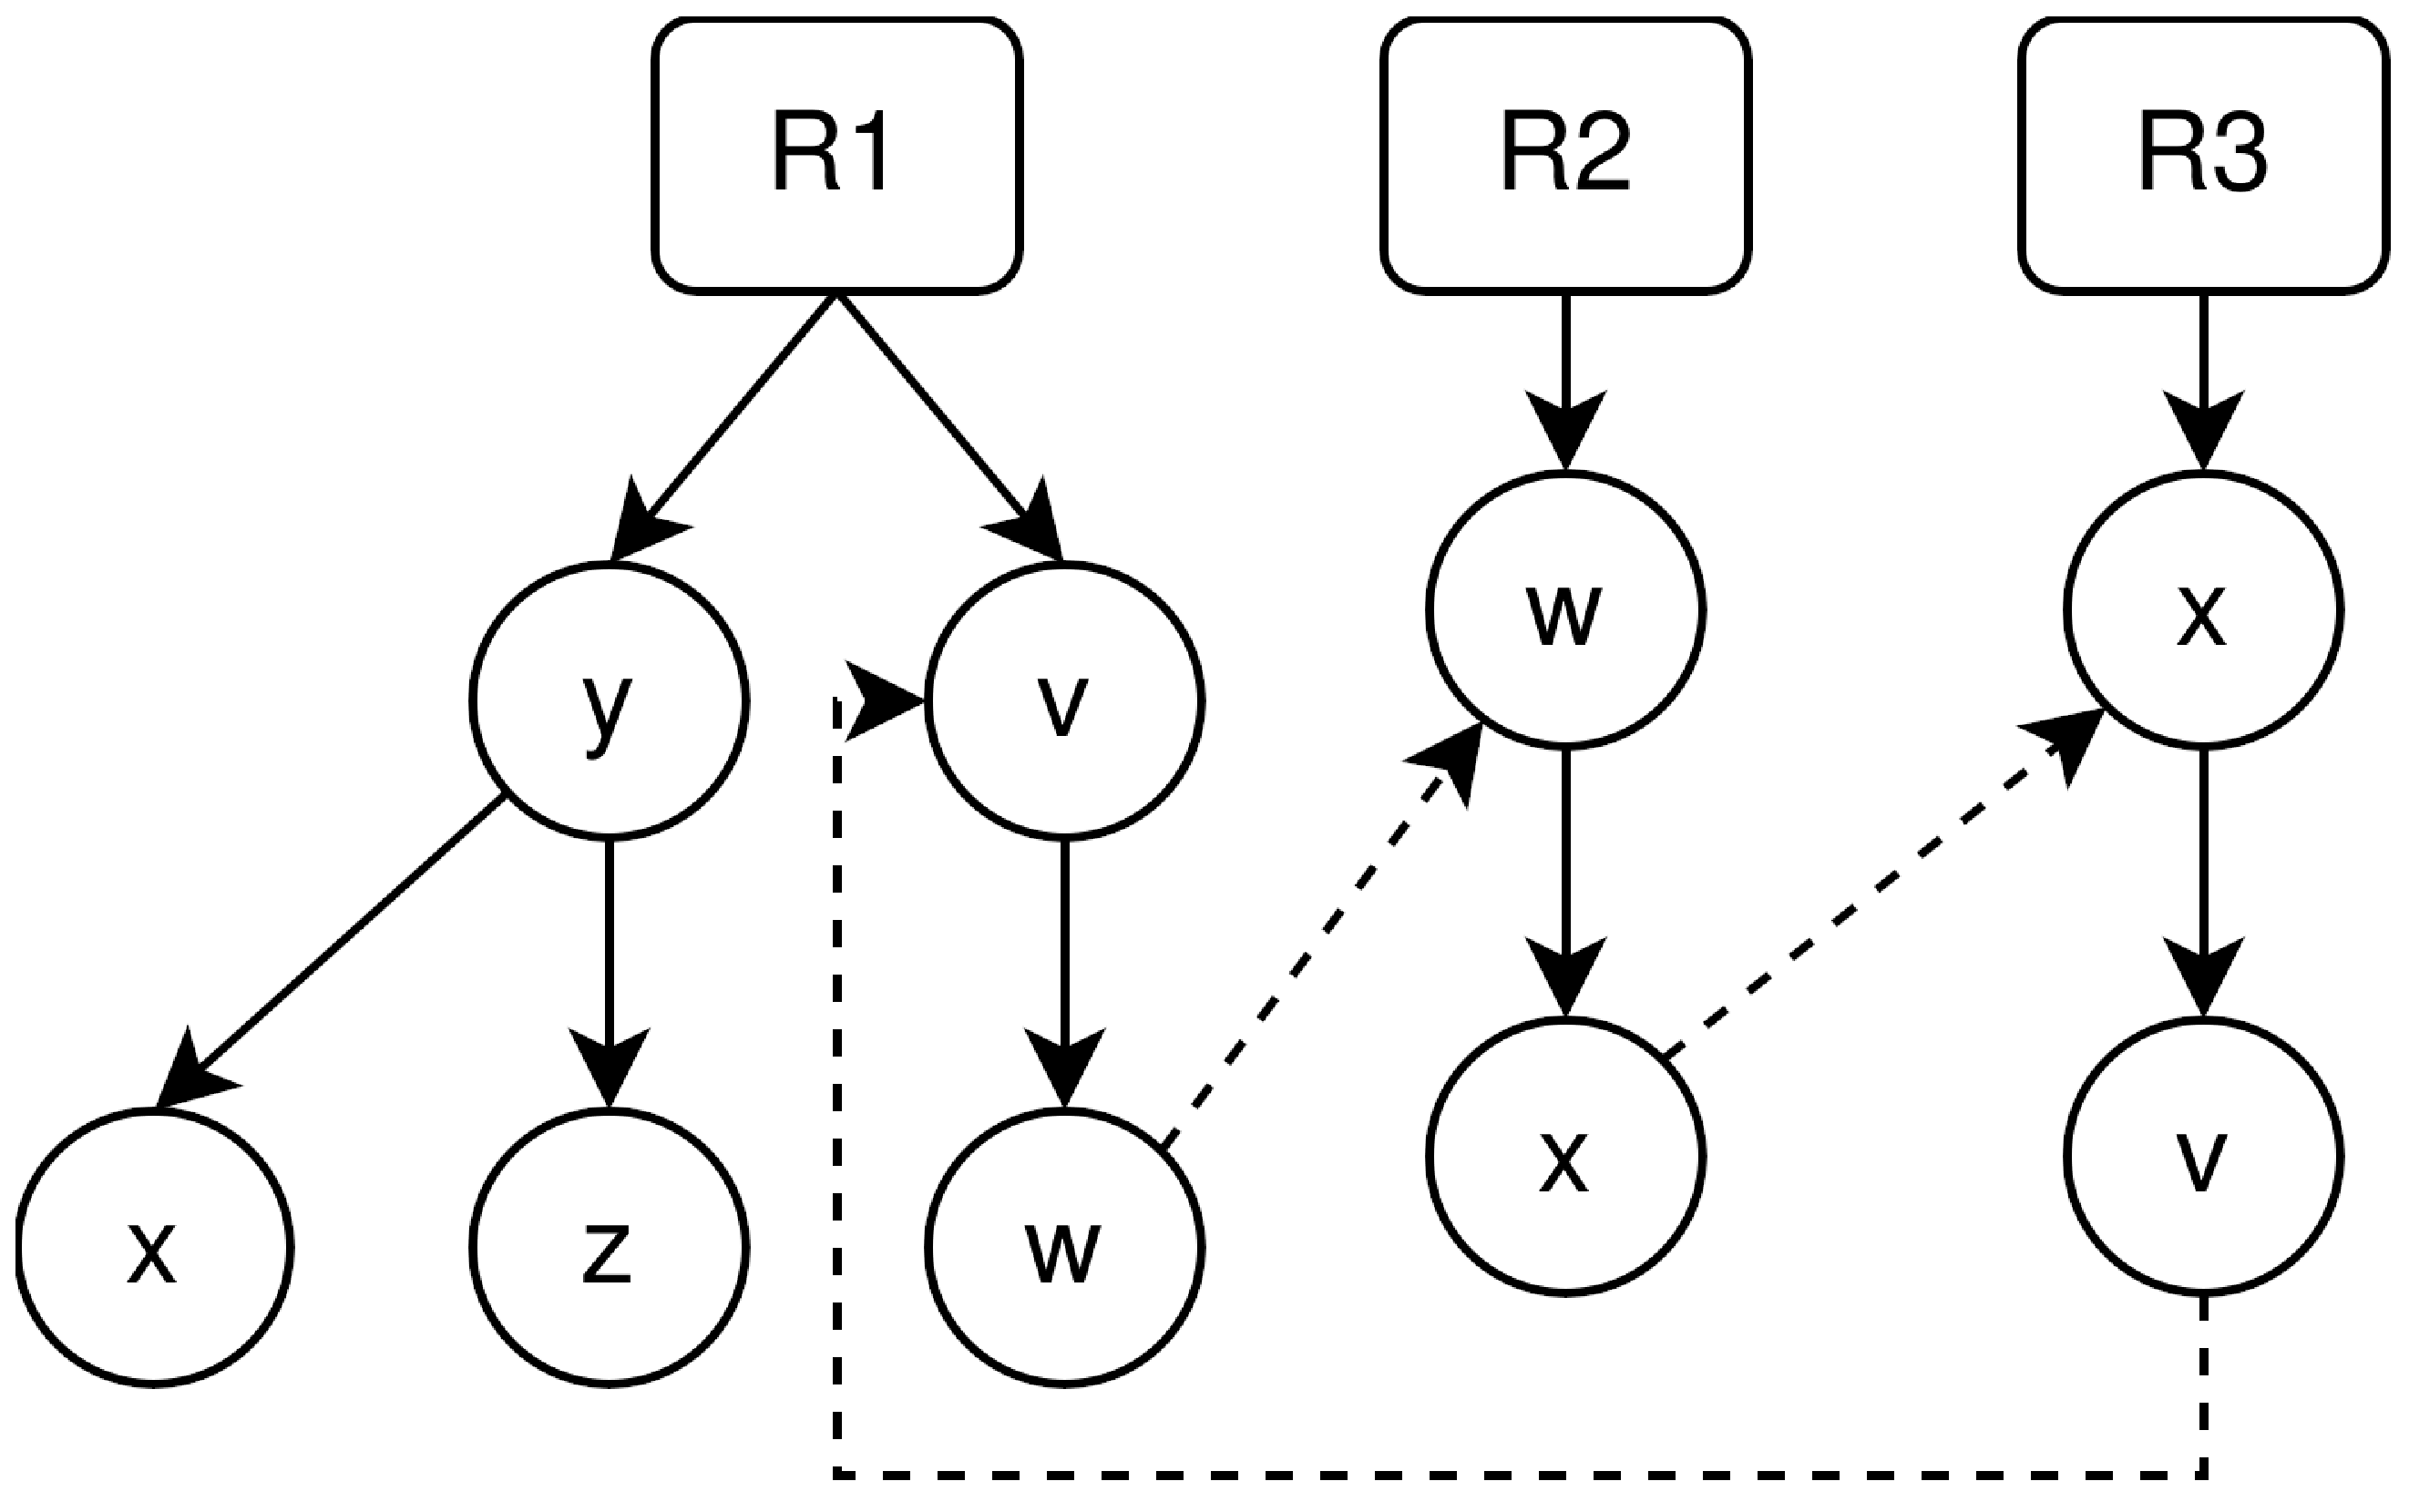
\includegraphics[width=0.5\textwidth]{img/tree_example.eps}
  \caption{Graphische Darstellung des Lock-Graphen für das Beispielprogramm in 
    Abb.~\ref{Chap:Analyze-Sec:Mutex-Fig:ZyclicTreeCode}. Durch die gestrichelten 
    Pfeile wird der enthaltenen Zyklus angezeigt.}
    \label{Chap:Analyze-Sec:Mutex-Fig:ZyclicTreeImg}
\end{figure}



\subsubsection{Channel}\label{Chap:Theo-Sec:Analyze-SubSec:Channel}
Man betrachte nun die Erkennung von Situationen, in denen eine Channel-Operation
zwar begonnen, aber nie ausgeführt worden ist. 
In diesen Fällen gibt es in dem Trace eine Channel-Information, 
welche ein Pre- aber kein Post-Event besitzt. Solch eine Situation bezeichnen wir als hängenden Channel. 
Solche hängenden 
Channel können auf einen potenziellen oder tatsächlich auftretenden Channel hindeuten.
Es sei allerdings auch hier dazu gesagt, dass eine solche hängende Operation nicht 
immer zu einem ``echten'' Deadlock führen muss.
Man betrachte dazu das Beispiel in Abb.~\ref{Chap:Analyze-Sec:Channel-SubSec:Dangling-Fig:ExDanglingWithout}.
\begin{figure}[h!]
  \lstinputlisting{code/example-dangling-without.txt}
  \caption{Hängender Channel ohne Deadlock}
  \label{Chap:Analyze-Sec:Channel-SubSec:Dangling-Fig:ExDanglingWithout}
\end{figure}
Da auf dem Channel \texttt{x} nie gesendet wird, kommt es es in Zeile~3 zu einer hängenden Channel-Operation. Da 
dabei aber die Main-Routine nicht blockiert wird, kommt es nicht zu einem Deadlock und die Go-Routine 
terminiert, sobald die Main-Routine terminiert. Solch eine Routine bezeichnen wir als leakende Routine.
Sie führt hierbei nicht zu einem Deadlock, ist aber in der Regel dennoch eine ungewollte Situation.
Es ist also sinnvoll, auch solche Situationen zu erkennen.\\\\
Um solche Situationen verhindern 
zu können, ist es sinnvoll, die möglichen Kommunikationspartner für diese 
Operation zu bestimmen um dem Nutzer bei der Suche und Beseitigung 
solcher Situationen zu helfen. Für Abb.~\ref{Chap:Analyze-Sec:Channel-SubSec:Dangling-Fig:ExDangling}
soll also angegeben werden können, dass die Send-Operation in 1 sowohl mit 2 als auch mit 3 
synchronisieren kann. Dabei sei allerdings zu beachten, dass nur weil eine Send- und eine 
Receive-Operation auf dem selben Channel und in unterschiedlichen Routine geschehen, nicht 
in jedem Fall eine Kommunikation zwischen diesen möglich ist. Man betrachte dazu das Beispiel in 
Abb.~\ref{Chap:Analyze-Sec:Channel-SubSec:Dangling-Fig:NoSync}.
\begin{figure}[h!]
  \lstinputlisting{code/example-no-sync.txt}
  \caption{Beispielprogramm für unmögliche Synchronisation}
  \label{Chap:Analyze-Sec:Channel-SubSec:Dangling-Fig:NoSync}
\end{figure}
Auf dem Channel \texttt{x} wird in 1 gesendet und kann in 2 und 3 empfangen werden. Da es zwei Receive, 
aber nur eine Send-Operation gibt, kommt es zu einem hängenden Channel. Betrachtet man nur 
Channel \texttt{x} könnte man davon ausgehen, dass 1 nach 2 senden kann, was zu einem Deadlock
führen würde. Dies ist aber nicht möglich. Da der Channel \texttt{y} in 1 nach \texttt{x} sendet, 
in 2 allerdings von \texttt{x} empfangen muss, ist eine Synchronisierung auf \texttt{x} von 1 nach 
2 nicht möglich. Die beiden Operationen bilden demnach keine möglichen Kommunikationspartner.\\\\
Um mögliche Kommunikationspartner zu erkennen, nicht mögliche Kommunikationspartner wie in 
Abb.~\ref{Chap:Analyze-Sec:Channel-SubSec:Dangling-Fig:NoSync} aber auszuschließen, werden
Vector-Clocks verwendet. Die grundlegende Idee basiert auf~\cite{PPDP18}.\\
In einem ersten Durchlauf wird dabei der Trace mit Vector-Clock Informationen nach der Methode 
von Fidge~\cite{Fidge} erweitert. Für jede Routine 
wird eine Vector-Clock gespeichert, welche für jede Routine einen Wert enthält. Zu Begin werden 
all diese Werte auf 0 gesetzt. Bei jedem Post-Event, sowohl für Send als auch Receive und für 
Signal und Wait Elemente wird der Wert der eigenen Routine in der lokalen Vector-Clock um eins 
erhöht. Bei einem Post-Receive und einem Wait Element wird die Vectorclock $vc'$ betrachtet, 
welche in der sendenden Routine zum Zeitpunkt des Post-Send- bzw. Signal-Elements vorlag. 
Da ein Send- bzw. Signal-Event immer vor dem Receive- bzw. Wait-Element erzeugt wird, wurde 
die entsprechende Vectorclock in jedem Fall bereits bestimmt. Die Zuordnung der Trace-Elemente 
ist möglich, da der globale Counter bei einem Send an den Empfangenden Channel mitgesendet 
wird, und in dem entsprechenden Post-Receive- bzw. Wait-Trace-Element gespeichert wird.
Bei einem Select-Statement wird nur derjenige Fall betrachtet, der auch tatsächlich ausgeführt wurde.
Diese Vector-Clock \texttt{vc}
wird nun mit der lokalen Vector-Clock $vc$ der empfangenden Routine, bzw. der Wait-Routine 
\texttt{q} verrechnet und ersetzt diese. Dabei gilt\\
\begin{figure}[h]
  \centering
  \lstinputlisting[frame=none, numbers=none]{code/vector-clock.txt}
\end{figure}\\
wobei $n$ die Anzahl der Routinen ist.\\
Für alle andern Elemente, z.B. Pre usw., wird einfach die lokale Vector-Clock der Routine übernommen, 
ohne diese zu verändern. Da nun die Vector-Clocks zu jedem Zeitpunk bestimmt wurde, kann jedem 
Send- und Receive-Trace-Element eine Pre- und eine Post-Vector-Clock zugeordnet werden. 
Dabei handelt es sich um die Vector-Clocks, die bei Erzeugung des Pre- bzw. Post-Events in 
der Routine, in der die Operation ausgeführt wurde vorlag. Für hängende Operationen, 
bei denen kein Post-Element existiert, werden alle Werte der Post-Vector-Clock auf 
max(Int32) gesetzt.
Man betrachte das Beispiel in Abb.~\ref{Chap:Analyze-Sec:Channel-SubSec:Dangling-Fig:PorgVC}.
\begin{figure}[h!]
  \centering
  \lstinputlisting{code/example-vector-clock-prog.txt}
  \caption{Beispielprogramm für die Betrachtung der Vector-Clocks}
  \label{Chap:Analyze-Sec:Channel-SubSec:Dangling-Fig:PorgVC}
\end{figure}
Man betrachte den Fall, in dem 3 mit 4 und dann 1 mit 5 synchronisiert und 2 eine hängende Operation bildet.
In diesem Fall erhält man folgenden Trace:
\begin{align*}
  [&[signal(1, 2), signal(2, 3), pre(1, x?), post(7, 1, x?, 6), pre(8, x?), post(13, 1, x?, 11)]\\
  &[wait(9, 2), pre(10, x!), post(11, 1, x!), pre(12, x?)]\\
  &[wait(4, 3), pre(5, x!), post(6, 2, x!)]
  ]
\end{align*}
Aus diesem Trace lassen sich nun die Vector-Clocks für die einzelnen Operationen berechnen.
Der Ablauf des Programs, welcher dem Trace entspricht, inklusive der Vector-Clocks 
ist in Abb.~\ref{Chap:Analyze-Sec:Channel-SubSec:Dangling-Fig:VC} gegeben.
\begin{figure}[h!]
  \centering
  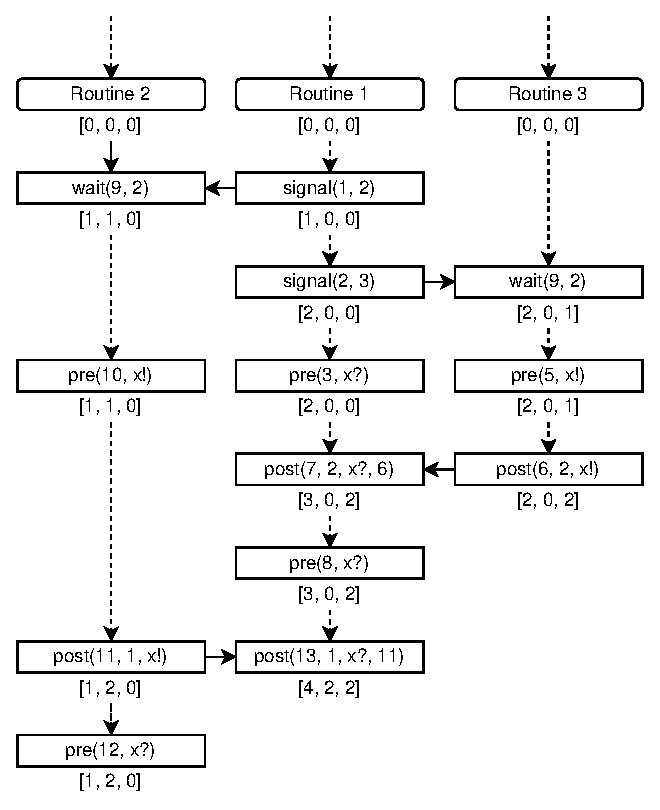
\includegraphics[width=0.5\textwidth]{img/vector_clock_graph.eps}
  \caption{Ablaufdiagramm mit Vector-Clocks für das Beispiel in Abb.~\ref{Chap:Analyze-Sec:Channel-SubSec:Dangling-Fig:PorgVC}}
  \label{Chap:Analyze-Sec:Channel-SubSec:Dangling-Fig:VC}
\end{figure}
Von diesen lassen sich nun die Pre- und Post-Vector-Clocks direkt ablesen.
Für den Vectorclock-Annotierte-Trace (VAT) werden diese in der Form $^{vc}a^{vc'}$ 
mit der Pre-Vector-Clock $vc$ und der 
Post-Vector-Clock $vc'$ und der Channel-Operation $a$ angegeben. Für Close gilt, 
dass die Pre-Vectorclock gleich der Post-Vectorclock ist. Andere Elemente 
werden in den VAT nicht aufgenommen, da sie 
für die anschließende Analyse nicht benötigt werden.
Der VAT gibt sich in diesem Fall also als
\begin{align*}
  [&[^{[2,0,0]}x?^{[3,0,2]}, ^{[3,0,2]}x?^{[4,2,2]}]\\
  &[^{[1, 1, 0]}x!^{[1, 2, 0]}, ^{[1, 2, 0]}x?^{[max, max, max]}]\\
  &[^{[2, 0, 1]}x!^{[2, 0, 2]}]]
\end{align*}
Man bezeichne zwei Vector-Clocks $vc$ und $vc'$ als vergleichbar, wenn
$\forall i: vc[i] \leq vc'[i]$ oder $\forall i: vc[i] \geq vc'[i]$. Man 
schreibe in diesem Fall $vc \leq vc$ bzw. $vc \geq vc$ bzw.~allgemein 
$vc \gtreqless vc'$. Andernfalls 
bezeichnen man $vc$ und $vc'$ als unvergleichbar $vc \not\gtreqless vc'$. 
Sind zwei Vector-Clocks 
unvergleichbar, sind sie unabhängig und können somit gleichzeitig auftreten. 
Man erkennt also zwei Operationen, welche eine mögliche Kommunikation durchführen 
können daran, dass sie auf dem selben Channel definiert sind, eine Send-
und eine Receive-Operation definieren und dass 
 ihre Pre- oder Vector-Clocks unvergleichbar sind.
Um alternative Kommunikationspartner für hängende Kanäle zu finden, werden also
die Pre- und Post-Vector-Clocks der Channels mit dem selben Channel verglichen.\\
Man betrachte die hängende Receive-Operation in dem obigen Beispiel. Es gibt 
in dem Programm 2 Send-Operationen, welche als Kommunikationspartner für 
die hängende Operation $r$ in Frage kommen. Vergleicht man die Vector-Clocks der 
Send-Operationen mit denen der hängenden Operation wird aber klar, dass nur 
eine der beiden Operationen tatsächlich möglich ist. Für die Send-Operation 
in der 2. Routine (der selben wie die hängende Operation) $s_1$ gilt 
$s_{1, pre} \leq r_{pre}$ und $s_{1, post} \leq r_{pre}$.  
Für die andere Send-Operation $s_2$ in Routine 3 hingegen gilt 
$s_{1, pre} \not\gtreqless r_{pre}$. Sie kann also gleichzeitig mit der 
hängenden Operation ausgeführt werden und bildet somit einen potenziellen 
Kommunikation. Hierbei wird auch klar, warum es nicht nur ausreicht einen 
Trace aufzuzeichnen, wenn eine Operation ausgeführt wird. Da für die 
Post-Vector-Clocks gilt, dass $s_{2, post} \geq r_{post}$, kann allein aus der 
Post-Vector-Clock nicht auf eine mögliche oder unmögliche Kommunikation geschlossen werden.\\\\
In gebufferten Channels ist nicht notwendig, dass Send und Receive gleichzeitig
ausgeführt werden.
Da der Trace somit bei einem Send ohne Receive, bzw.~einem Receive ohne gleichzeitigem
Send ein gültiges Post-Event besitzt, 
wird dieses Problem nicht direkt erkannt.\\
Situationen, bei denen gesendet Nachrichten auf einem Channel 
nie ausgelesen werden, lassen sich aus dem Trace erkennen.
Dazu wird der mit Vector-Clocks annotierte Trace durchlaufen. Auf diesem 
wird nun für jeden Channel gezählt, wie oft erfolgreich gesendet bzw. erfolgreich empfangen 
wurde (Anzahl der entsprechenden Elemente, bei denen die Post-Vector-Clock 
nicht max(Int) ist). Ist die Anzahl der erfolgreichen Send größer als 
die Anzahl der erfolgreichen Receive, bedeutet diese, dass nach Abschluss des 
Programms auf dem entsprechenden Channel noch nicht gelesene Nachrichten vorhanden sind.\\
\begin{figure}[h!]
  \centering
  \lstinputlisting{code/buffered_not_possible.txt}
  \caption{Beispielprogramm für die Betrachtung der Vector-Clocks}
  \label{Chap:Analyze-Sec:Channel-SubSec:Dangling-Fig:BufferedNoSync}
\end{figure}
Theoretisch ist es einem gebufferten Channel möglich bei einem Send mit 
jedem Receive auf dem selben Channel zu kommunizieren, welches nicht 
streng vor dem Send ausgeführt werden muss. In der Praxis geben sich allerdings 
Situationen in welchen eine Synchronisation zwischen Send- und Receive nicht 
möglich ist. Man betrachte dazu das Beispiel in 
Abb.~\ref{Chap:Analyze-Sec:Channel-SubSec:Dangling-Fig:BufferedNoSync}.
Auf den ersten Blick scheint es möglich, dass alle Send (1-4) mit allen 
Receive (5-9) kommunizieren könnten. Dies ist aber nicht der Fall.
Angenommen 1 und 2 senden, bevor es zu einem Receive kommt. Da gebufferte 
Channel in der Praxis wie FIFO Queue funktionieren, kann 2 nicht mit 5 
Synchronisieren, da bei dem Receive auf 5 zuerst der Wert aus 1 empfangen 
werden würde. Um bestimmen zu können, auf welchen Operationen eines 
gebufferten Channel tatsächlich das eine Kommunikation möglich ist, 
werden für jedes Paar von Send-Receive Operationen die folgenden Werte aus 
dem VAT bestimmt: 
\begin{itemize}
  \item $S_p$: Anzahl der Send Operationen, vor der betrachteten Send-Operation 
    in der selben Routine ausgeführt werden,
  \item $S_u$: Anzahl der Send-Operationen, welche unvergleichbar mit der 
    betrachteten Send-Operation sind,
  \item $R_p$: Anzahl der Receive Operationen, vor der betrachteten Receive-Operation 
    in der selben Routine ausgeführt werden,
  \item $R_u$: Anzahl der Receive-Operationen, welche unvergleichbar mit der 
    betrachteten Receive-Operation sind.
\end{itemize}
Ein Paar von Send-Receive Operationen werden nun genau dann als mögliche 
Kommunikationspartner gesehen, wenn 
\begin{align}
  S_p &\leq R_p - R_u  \label{Form:1}\\
  \text{und }\qquad S_p +  S_u &\geq R_p + R_u \label{Form:2}
\end{align}
Nachdem nun alle möglichen Kommunikationspartner ermittelt wurden, 
können die möglichen Ausführungspfade betrachtet werden, um zu überprüfen, 
ob diese zu Problemen führen. Der Detektor geht dazu alle vorhandenen Send-Operationen 
durch und ordnet Schrittweise jeder Operation eine Receive-Operation zu, so dass 
die Send- und Receive-Operation potenzielle Kommunikationspartner 
bilde und keine zwei Send-Operationen die selbe Receive-Operation 
besitzen. Es kann nun vorkommen, dass ein Teil der Send-Operationen bereits eine 
Receive-Operation zugeordnet bekommen haben, einer weiteren Send-Operation 
aber kein gültiges Receive zugeordnet werden kann. Dies bedeutet, dass 
wenn der Ablauf des Programm wie in den bereits zugeordneten Paaren geschieht, die Operation, 
welcher keine gültige Receive-Operation zugeordnet werden kann, keinen 
gültigen Kommunikationspartner besitzt. Dies bedeutet, dass es zu einem 
Deadlock, einer hängenden Routine, oder einer nicht ausgelesenen Nachricht 
in einem gebufferten Channel kommt. In diesem Fall wird eine Warnung 
mit den entsprechenden Informationen ausgegeben. Das selbe wird auch umgekehrt durchgeführt. Es wird als 
versucht jeder Receive-Operation eine Send-Operation zuzuordnen. 
Auch hier kann eine Situation, in welcher keine gültige Zuordnung für eine
der Operationen möglich ist, zu einem Bug führen.\\
Nicht alle so betrachteten Ordnungen bilden gültige Ordnungen. Man betrachte 
dazu erneut Abb.~\ref{Chap:Analyze-Sec:Channel-SubSec:Dangling-Fig:PorgVC}. 
Es ist hierbei prinzipiell möglich, dass 2 mit 6 kommuniziert. Wenn 
allerdings 3 mit 5 kommuniziert ist dies nicht möglich, da 1 vor 2 kommunizieren 
muss und daher eine Kommunikation zwischen 2 und 6 nicht mehr möglich ist. 
Eine Ausführungsordnung sei daher nur dann gültig, wenn für jede Operation $O$ 
welche in der Ordnung betrachtet wird auch alle anderen Operationen aus 
der selben Routine, welche vor $O$ ausgeführt werden in der Ausführungsordnung 
vorhanden sind.



\subsubsection{Close}
Versuch ein Programm auf einem geschlossenen Channel zu senden kommt es zu einem Laufzeitfehler, 
welcher in einem Programmabbruch führt. Solch eine Situation lässt sich 
dadurch erkennen, dass eine Close- und eine Send-Operation auf dem selben Channel
gleichzeitig ablaufen können, dass also die Pre- oder Post-Vectorclock 
der Send-Operation unvergleichbar mit der Vectorclock der Close-Operation 
ist. Situationen, bei denen die Vectorclocks der Send-Operation streng später 
als die der Close-Operation sind führen immer dazu, das es zu einem einem 
Send auf einem geschlossenen Channel kommt. In diesem Fall kommt es also immer 
zu einem Laufzeitfehler des Programms, durch welchen das Programm abgebrochen wird.

\subsection{Select}\label{Chap:Back-Sec:Select}
In Go können Select-Statements dazu verwendet werden, abhängig davon, 
auf welchen Channels Nachrichten gesendet werden unterschiedliche Programmteile
auszuführen. Dies erschwert die Analyse des Programs, da der 
tatsächliche Programmablauf dabei praktisch nicht-deterministisch werden 
kann~\cite{select-spec}. Da der aufgezeichnete Trace immer nur einen 
Programmablauf betrachtet, führt dies zu Problemen, da 
nicht betrachtete Ausführungspfade zu Deadlocks oder anderen Problemen 
führen können. Eine Möglichkeit besteht darin, das Programm mehrfach auszuführen, 
und dabei immer unterschiedliche Select-Cases zu erzwingen. Ein solcher 
Ansatz wird unter anderem in~\cite{gfuzz} verwendet. Dazu werden die 
Select-Statements in dem Programmcode so verändert, dass aus den vorhandenen 
Cases eines gezielt bevorzugt werden kann.
Der Ablauf eines Programms bezüglich seiner 
Select-Statements kann nun als Liste von Tupeln 
$[(s_0, c_0, e_0), \ldots, (s_n, c_n, e_n)]$ dargestellt werden. Dabei 
bezeichnet $s_i (0 \leq i \leq n)$ die ID einer Select-Operation, $c_i$ 
die Anzahl der Cases in dieser Operation und $e_n$ den Index des Ausgeführten 
Case. Das Programm wird nun mehrfach durchlaufen, wobei die Ordnung zufällig 
verändert wird. Dazu wird nach jedem Durchlauf der Index $e_i$ jedes Tupels 
auf einen zufälligen, aber gültigen Wert gesetzt. Da die Anzahl der möglichen 
Ausführungspfade durch die Select-Statements gegebenenfalls gegen unendlich gehen kann,
ist es nicht möglich jede mögliche Kombination von Select-Cases auszuführen.
Aus diesem Grund sammelt GFuzz während der Ausführung einer Ordnung Informationen 
über diese, um die Qualität einer Ordnung abzuschätzen. Aus diesen wird 
eine Wertung für die durchlaufenden Ordnung bestimmt, über welche die 
Anzahl der Mutationen bestimmt werden. \\\\
Die Betrachtung von verschiedenen Pfaden von Select wird auch für GoChan 
verwendet. Für jeden Durchlauf wird 
der Trace aufgezeichnet und dieser
analysiert. Die Auswahl der Pfade wird dabei vereinfacht. Anders als 
in GFuzz basieren die betrachteten Ausführungsordnungen nicht auf schon versuchten Ordnungen,
sondern es wird eine Menge von vollständig zufälligen Ordnungen betrachtet.
Die Sammlung von Informationen über die einzelnen Abläufe bedeutet einen 
deutlichen Mehraufwand, sowohl bei der Implementierung, als auch bei der eigentlichen 
Bestimmung der für die Abschätzung benötigten Werte. Da der Nutzen dabei eher gering ist,
wird darauf verzichtet.
